\documentclass[a4paper,12pt]{article}
\usepackage[utf8]{inputenc}
\usepackage{graphicx}
\usepackage{textcomp}
\usepackage{gensymb}
\usepackage{cancel}
\usepackage{fancyhdr}
\usepackage{siunitx}
\usepackage{float}
\usepackage[labelfont=bf]{caption}
\usepackage[colorlinks=true,linkcolor=blue,urlcolor=black,bookmarksopen=true]{hyperref}
\usepackage{subcaption}
\usepackage{amsmath}
\usepackage{amssymb}
\usepackage{booktabs}
\usepackage{bm}
\usepackage[margin=1in]{geometry}

\usepackage[english]{babel}
\usepackage{amsthm}
\usepackage[noabbrev,capitalize,nameinlink]{cleveref}

\usepackage{enumitem}

\theoremstyle{plain}
\newtheorem*{thm}{Theorem}
\newtheorem*{cor}{Corollary}
\newtheorem{lem}{Lemma}
\newtheorem*{ax}{Axiom}

\theoremstyle{definition}
\newtheorem{definition}{Definition}
\newtheorem*{ex}{Example}
\newtheorem*{soln}{Solution}

\theoremstyle{remark}
\newtheorem*{rmk}{Remark}

\setlength{\parindent}{5ex}
\setlength{\headheight}{22pt}

\pagestyle{fancy}
\fancyhf{}
\rhead{CTA200} % Course Code
\lhead{Ian Niebres} % Name
\chead{\Large{\textbf{Assignment 3}}} % Title (Problem Set #)

\title{CTA200 2022 Assignment 3} % Title again
\author{DUE: Tuesday May 10th by 1:00 PM} % due date
\date{} 

\begin{document}
\maketitle
\section*{Question 1}
%------------------------------------------------------------------%
%                           Question 1                             %
%------------------------------------------------------------------%
In this question, we iterated the equation $z_{n+1} = z_n^{\; 2} + c$ for
each point $c = x+iy$ in the complex plane for $-2 < x < 2$ and 
$-2 < y < 2$. A function called \texttt{iterate} was written
in the file \texttt{iteration.py} which performs this iteration
\texttt{N} times given an initial $z_0 = 0$ and $c = x+iy$. 

\begin{figure}[H]
    \centering
    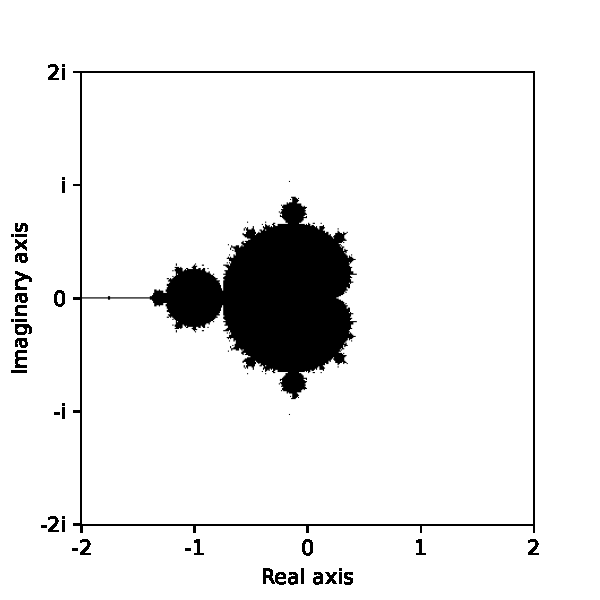
\includegraphics[width=0.8\linewidth]{../plots/a3q1_1.pdf}
    \caption{}
\end{figure}

\section*{Question 2}
%------------------------------------------------------------------%
%                           Question 2                             %
%------------------------------------------------------------------%

\section*{Question 3}
%------------------------------------------------------------------%
%                           Question 3                             %
%------------------------------------------------------------------%

\end{document}